\documentclass{standalone}
\usepackage{tikz-feynman}

\begin{document}
    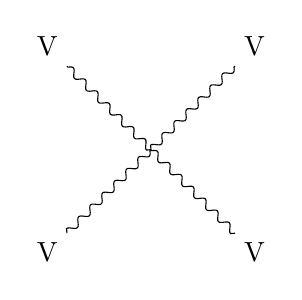
\begin{tikzpicture}[baseline={(current bounding box.center)}]
    \begin{feynman}
    \vertex (a) ;
    \vertex [above   left=of a] (c) {V};
    \vertex [below   left=of a] (d) {V};
    \vertex [above right=of a] (e) {V};
    \vertex [below right=of a] (f) {V};
    \diagram* {
        (c) -- [boson] (a) -- [boson] (d),
        (e) -- [boson] (a) -- [boson] (f),
    };
    \end{feynman}
    \end{tikzpicture}
\end{document}